\documentclass[12pt,a4paper,preprint]{elsarticle}
\usepackage[utf8]{inputenc}
\usepackage[english]{babel}
\usepackage[a4paper,left=2cm,right=2cm,top=2cm,bottom=2.7cm]{geometry}
\usepackage{amsmath,amssymb,amsfonts,amsthm,bm,graphicx,booktabs,multirow,array,tabularx,xcolor,hyperref}

\makeatletter
\def\ps@pprintTitle{%
    \let\@mkboth\markboth
    \def\@evenhead{%
        \ifnum\c@page>1
            {\footnotesize\thepage}\hfil{\footnotesize\itshape\leftmark}%
        \fi}%
    \def\@oddfoot{\footnotesize\itshape
        Preprint\hfill\thepage\relax}%
    \let\@evenfoot\@oddfoot
}
\AtBeginDocument{\pagestyle{pprintTitle}}
\makeatother
\graphicspath{{figs/}}

\begin{document}
    \begin{frontmatter}
        \title{Macroscopic quantum tunneling between\\acoustic black and white holes in the Michel flow}
        \author{Alexander V. Semyannikov}
        \address{Independent Researcher \\ \textit{Email: avsemyannikov@gmail.com}}
        
        \begin{abstract}
            The relativistic Michel flow possesses two degenerate stationary solutions: the accretion branch ($\upsilon < 0$), which forms an acoustic black hole, and the wind branch ($\upsilon > 0$), which forms an acoustic white hole. Both solutions are stationary points of a single energy functional; the barrier between them is of inertial origin and is due to the necessity of stopping and reversing the macroscopic flow. Within a one-parameter model reduction, an instanton trajectory in Euclidean time is constructed, connecting the two branches through the saddle point of the phase space. The instanton action is expressed through the effective moment of inertia of the flow and the height of the energy barrier; both factors are finite owing to the convergence of the integral with the $\upsilon^{2}$ factor. Numerical estimates for $a_{\infty} \in \{0.05,\, 0.1\}$ show that the instanton action is controlled by the macroscopic scales of the acoustic horizon. The transition probability is exponentially suppressed and acquires physical meaning only for systems with a quantum microstructure ($\hbar_{\mathrm{eff}} > 0$). The detailed balance between the forward and reverse transitions is broken owing to the classical instability of the acoustic white hole. The construction is consistent with the invariant quantities established in the companion studies.
        \end{abstract}
        
        \begin{keyword}
            Michel accretion \sep analogue gravity \sep acoustic black hole \sep acoustic white hole \sep macroscopic quantum tunneling \sep instanton \sep Painlev\'e--Gullstrand coordinates \sep surface gravity \sep Hawking radiation \sep Bose--Einstein condensate
        \end{keyword}
    \end{frontmatter}

    \section{Introduction}\label{sec:introduction}
        Acoustic perturbations in a moving fluid propagate on an effective Lorentzian geometry constructed from the background spacetime metric, the flow 4-velocity, and the local speed of sound~\cite{UnruhWG_ExperimentalBlackHoleEvaporation_1981, VisserM_AcousticBlackHolesHorizonsErgospheresAndHawkingRadiation_1998, BarceloC_LiberatiS_VisserM_AnalogueGravity_2011}. For stationary spherical accretion onto a Schwarzschild black hole --- the Michel flow~\cite{MichelFC_AccretionOfMatterByCondensedObjects_1972} --- this construction generates an acoustic horizon coinciding with the critical point of the flow~\cite{SemyannikovAV_AcousticGeometryAndSoundRayDynamicsInRelativisticSphericalAccretion_2026}. The geometric-optics phenomenology of sound rays in the exterior subsonic region was constructed in~\cite{SemyannikovAV_AcousticGeometryAndSoundRayDynamicsInRelativisticSphericalAccretion_2026}; the spectrum of finite-frequency perturbations and the regularization of the spatial problem by the acoustic horizon were established in~\cite{SemyannikovAV_PerturbationSpectrumOfMichelFlowAcousticVorticalAndEntropyModes_2026}; the global PG construction, regular at both horizons, was developed in~\cite{SemyannikovAV_GlobalAcousticGeometryOfMichelFlowInPainleveGullstrandCoordinates_2026}.
        
        A structurally parallel line of research, most explicitly developed by Volovik~\cite{VolovikGE_PainleveGullstrandCoordinatesForSchwarzschildDeSitterSpacetime_2023}, addresses the relation between the black-hole and white-hole states within a unified formalism. In the extended description of the Schwarzschild--de~Sitter spacetime in Painlev\'{e}--Gullstrand (PG) coordinates, the shift function changes sign at a stationary point, and the nine realizations of the configuration --- including black and white holes, contracting and expanding cosmologies --- turn out to be connected by singular coordinate transformations at the horizons. These transformations, although singular only in the coordinate sense, are interpreted as describing macroscopic quantum tunneling between physically inequivalent vacuum states, with the tunneling exponent related to the difference of their entropies. The transition from a black hole to a white hole is thereby formulated as a topological quantum process, rather than as an instability of a single classical solution.
        
        The Michel flow carries an exact hydrodynamic analogue of this structure. The stationary transonic solution is singled out by the simultaneous vanishing of the numerator and the denominator of $\mathrm{d}\upsilon/\mathrm{d}r$, which identifies the sonic point as a saddle in the phase plane $(\upsilon, r)$. The accretion branch, $\upsilon < 0$, passes smoothly from subsonic conditions at infinity to supersonic conditions at the horizon and gives rise to an acoustic black hole; the wind branch, $\upsilon > 0$, passes through the same saddle in the opposite direction and gives rise to an acoustic white hole. Both branches have identical integrals of motion and identical thermodynamic parameters, yet they are separated by a classically forbidden region: any continuous evolution from one branch to the other would require the fluid to linger indefinitely at the saddle point. This separation is the hydrodynamic analogue of the black/white hole dichotomy in vacuum gravity.
        
        In the present work, macroscopic quantum tunneling between the acoustic black-hole and acoustic white-hole states in the Michel flow is formulated and estimated. The PG representation developed in~\cite{SemyannikovAV_GlobalAcousticGeometryOfMichelFlowInPainleveGullstrandCoordinates_2026} is extended to both branches within a single smooth coordinate chart, and the instanton action governing the transition is expressed through the hydrodynamic variables of the flow. The tunneling exponent is related to the formal area of the acoustic horizon and to the surface gravity $\kappa$, thereby connecting the macroscopic transition with the kinematic Hawking scale established in the previous works. The result constitutes a quantitative realization --- within relativistic hydrodynamics --- of the black--white hole tunneling mechanism originally proposed for vacuum spacetimes.

    \section{Accretion--wind duality and the saddle structure of the Michel flow}\label{sec:duality}
        Throughout the work, the system of units $G = c = 1$ is used; lengths are dimensionless and measured in units of the gravitational radius $r_{\mathrm{g}}$; velocities and the speed of sound are in units of $c$; thermodynamic variables are normalized to their asymptotic values in the rest frame in accordance with the standard convention for the Michel flow~\cite{MichelFC_AccretionOfMatterByCondensedObjects_1972, MoncriefV_StabilityOfStationarySphericalAccretionOntoASchwarzschildBlackHole_1980}; the subscripts ``$\infty$'', ``c'', ``g'', and ``a'' denote the asymptotic value at infinity, the critical point, the gravitational horizon, and the acoustic horizon, respectively.
        \subsection{Michel integrals and the critical point}\label{subsec:michel-integrals}
            The background spacetime is described by the Schwarzschild metric
            \begin{equation}
                \mathrm{d}s^{2} = -f\,\mathrm{d}t^{2} + f^{-1}\,\mathrm{d}r^{2} + r^{2}\bigl(\mathrm{d}\theta^{2}+\sin^{2}\theta\,\mathrm{d}\phi^{2}\bigr), \qquad f(r) = 1 - \frac{1}{r},
                \label{eq:schwarzschild-metric}
            \end{equation}
            with the gravitational horizon at $r = 1$. The stationary spherically symmetric flow of a perfect fluid~\cite{MichelFC_AccretionOfMatterByCondensedObjects_1972} is characterized by a 4-velocity with temporal $\vartheta$ and radial $\upsilon$ components:
            \begin{equation}
                u^{\mu} = (\vartheta,\,\upsilon,\,0,\,0), \qquad f\vartheta = \sqrt{f + \upsilon^{2}}, \qquad \upsilon < 0,
                \label{eq:four-velocity}
            \end{equation}
            where $\vartheta$ is the temporal component, $\upsilon$ is the radial 3-velocity, and the condition $\upsilon < 0$ selects the accretion branch. The background is fixed by two first integrals, where $n$ is the particle number density, $h$ is the specific enthalpy, and $\mathcal{J}$ is the baryon flux:
            \begin{equation}
                r^{2} n \upsilon = \mathcal{J}, \qquad h\sqrt{f + \upsilon^{2}} = h_{\infty}.
                \label{eq:michel-integrals}
            \end{equation}
            The first integral expresses the conservation of the baryon flux through a spherical surface; the second expresses the conservation of the specific energy along a streamline and serves as the relativistic analogue of the Bernoulli equation. Together with the polytropic equation of state $p = K n^{\gamma}$, these relations determine the hydrodynamic profiles $\upsilon(r)$ and $a(r)$ for a given adiabatic index $\gamma$ and asymptotic sound speed $a_{\infty}$.
            
            A smooth transonic transition through the critical point $r_{\mathrm{c}}$ requires the simultaneous vanishing of the numerator and the denominator of $\mathrm{d}\upsilon/\mathrm{d}r$, which yields the standard conditions~\cite{ShapiroSL_TeukolskySA_BlackHolesWhiteDwarfsAndNeutronStarsThePhysicsOfCompactObjects_2004}:
            \begin{equation}
                \upsilon_{\mathrm{c}}^{2} = \frac{1}{4r_{\mathrm{c}}}, \qquad a_{\mathrm{c}}^{2} = \frac{\upsilon_{\mathrm{c}}^{2}}{1 - 3\upsilon_{\mathrm{c}}^{2}}.
                \label{eq:critical-point}
            \end{equation}
            These conditions single out the critical point as a saddle in the phase space $(\upsilon, r)$ and fix the unique physically regular accretion branch, which smoothly passes through the sound barrier from the subsonic regime at infinity to the supersonic regime at the horizon. The topology of the stationary solutions in the $(r, \mathcal{M})$ plane, where $\mathcal{M}$ is the physical Mach number measured by a locally static observer, was established in~\cite{SemyannikovAV_PerturbationSpectrumOfMichelFlowAcousticVorticalAndEntropyModes_2026}: at a fixed Bernoulli integral, each solution is a level line of the flux $\mathcal{J}$, and the critical flux corresponds to the unique transonic pair of branches intersecting at the sonic point.

            \begin{figure}[htb]
                \centering
                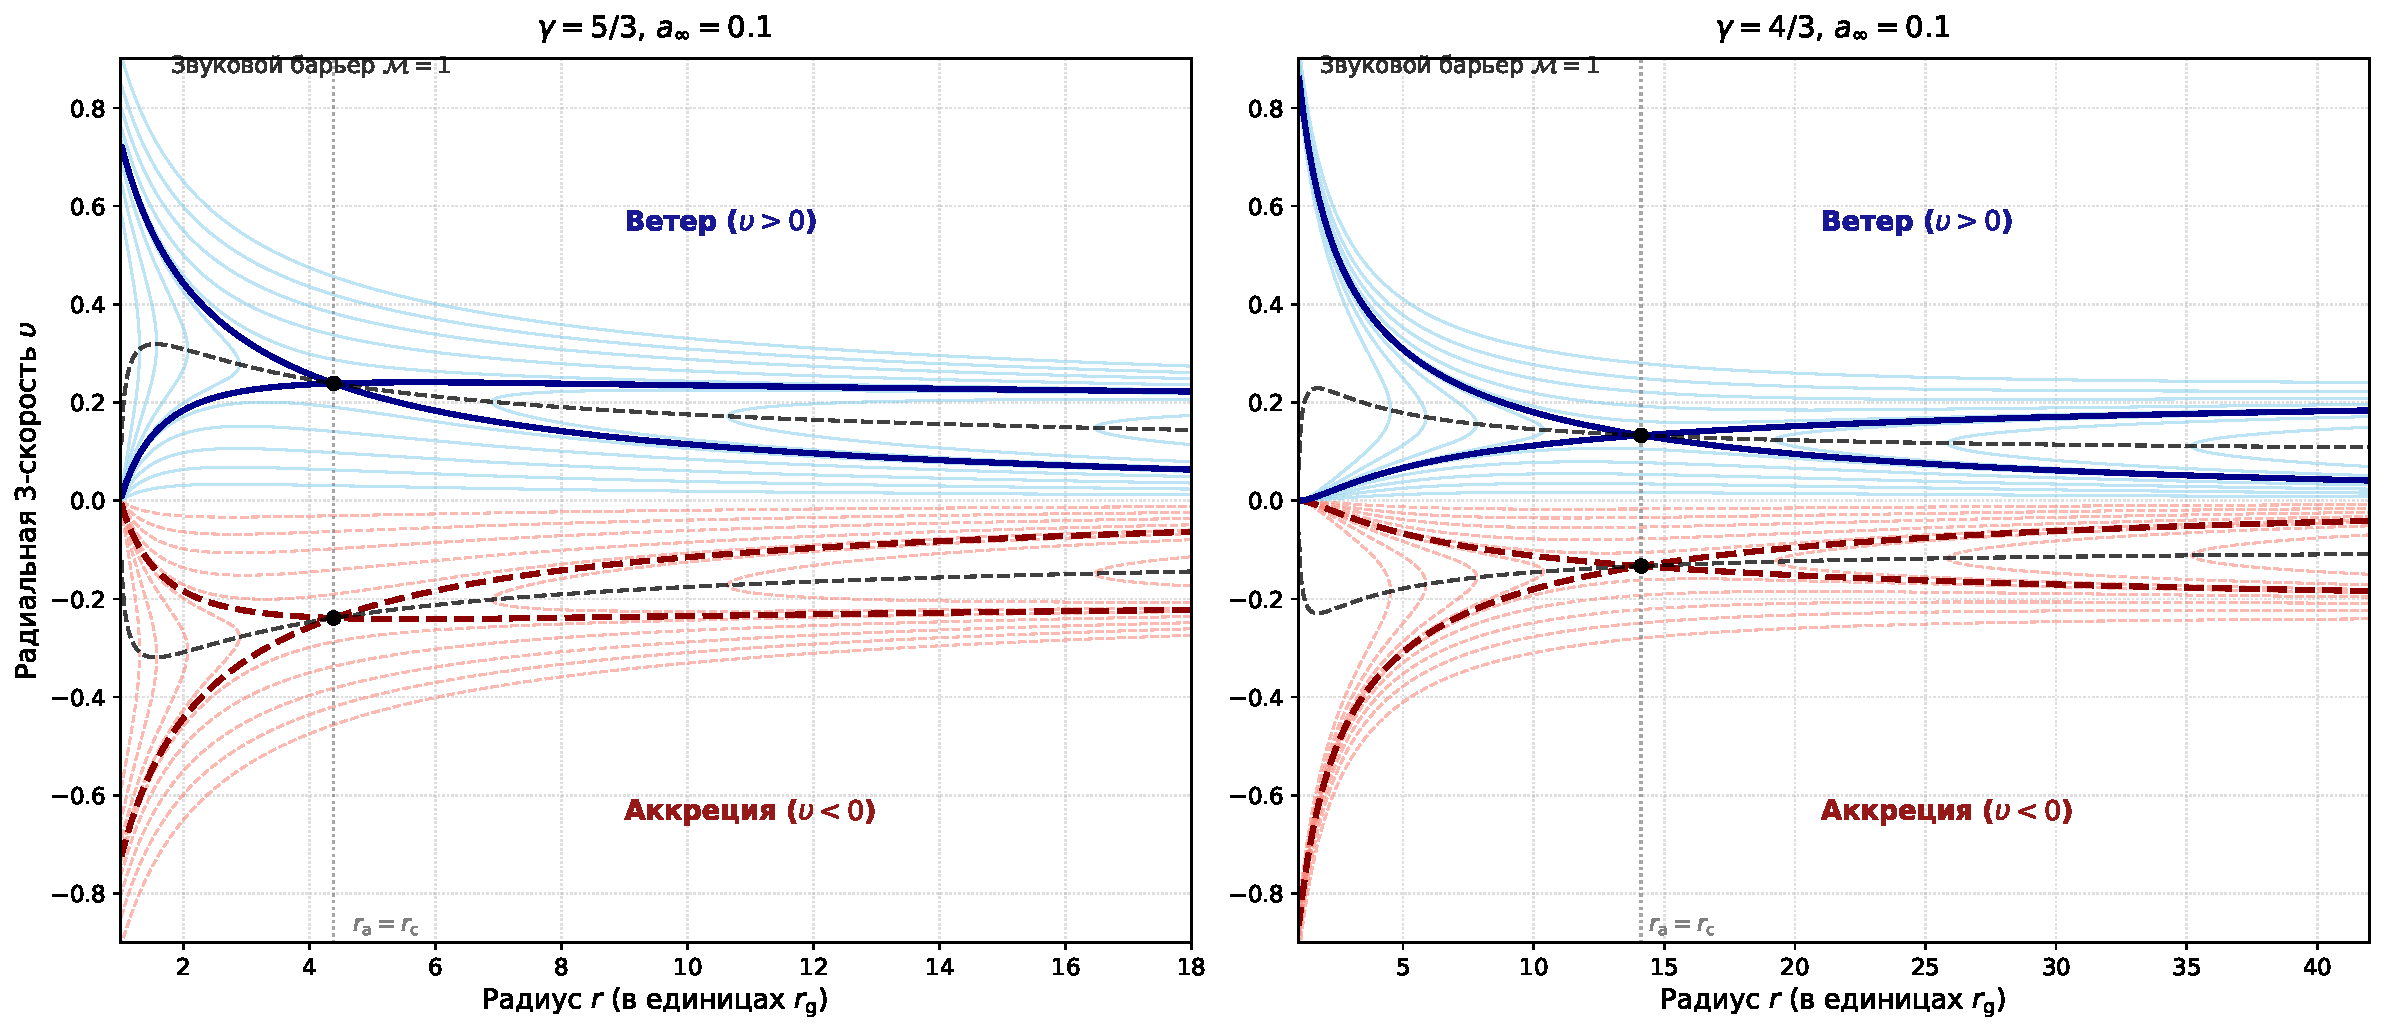
\includegraphics[width=\linewidth]{fig_phase_topology.pdf}
                \caption{Topology of the stationary solutions in the $(r, \mathcal{M})$ plane, where $\mathcal{M}$ is the physical Mach number measured by a locally static observer. At a fixed Bernoulli integral, each solution is a level line of the baryon flux $\mathcal{J}$. The critical flux corresponds to the unique transonic pair of branches (accretion, $\upsilon < 0$, and wind, $\upsilon > 0$) intersecting at the saddle sonic point $r = r_{\mathrm{c}}$. The horizontal solid black lines mark the sonic barrier $|\mathcal{M}| = 1$, which coincides with the acoustic horizon $r = r_{\mathrm{a}}$.}
                \label{fig:phase-topology}
            \end{figure}
            
            The analysis relies on the following assumptions: (i) stationarity and spherical symmetry of the background; (ii) a perfect fluid model with a polytropic equation of state; (iii) the absence of rotation and self-gravity of the accreting matter; (iv) the geometric-optics approximation for linear perturbations.

        \subsection{Two time-reversed branches}\label{subsec:two-branches}
            The saddle structure of the critical point~\eqref{eq:critical-point} implies the existence of two physically regular branches possessing identical integrals of motion~\eqref{eq:michel-integrals} and identical thermodynamic closure:
            \begin{itemize}
                \item \emph{Accretion branch}, $\upsilon < 0$, in which the flow accelerates inward from the state of rest at infinity, crosses the sound barrier at $r = r_{\mathrm{c}}$, and becomes supersonic inside the acoustic horizon. This branch constitutes the classical Michel flow and gives rise to an acoustic black hole.
                \item \emph{Wind branch}, $\upsilon > 0$, in which the flow emerges supersonically from the acoustic horizon, decelerates outward through the sonic point, and comes to rest at infinity. This branch is the exact time reversal of the accretion branch and gives rise to an acoustic white hole.
            \end{itemize}
            Both branches satisfy the same acoustic-horizon condition $\eta^{rr}(r_{\mathrm{a}}) = 0$, with $r_{\mathrm{a}} = r_{\mathrm{c}}$, and both possess the same surface gravity $\kappa$ and the same formal area of the acoustic horizon $\mathcal{A}_{\mathrm{a}}$~\cite{SemyannikovAV_AcousticGeometryAndSoundRayDynamicsInRelativisticSphericalAccretion_2026}. The two states are thus thermodynamically degenerate in the kinematic sense, yet they are separated by a classically forbidden region.
            
            The classical forbiddenness of the transition is a direct consequence of the conservation laws. The baryon flux $\mathcal{J} = r^{2} n \upsilon$ must remain constant along any classical trajectory; a continuous path from the accretion branch ($\mathcal{J} < 0$) to the wind branch ($\mathcal{J} > 0$) would require a change of the sign of $\mathcal{J}$, which is impossible without violating the baryon conservation law or passing through a singular state in which $n \to \infty$ or $\upsilon = 0$ everywhere. The only regular path connecting the two branches passes through the saddle point, where $\upsilon = \upsilon_{\mathrm{c}} \neq 0$, but this path requires the flow to linger indefinitely at the saddle, which is classically forbidden for a stationary configuration.
            
            The causal structures of the two branches are exact time reversals of each other~\cite{SemyannikovAV_GlobalAcousticGeometryOfMichelFlowInPainleveGullstrandCoordinates_2026}. For the accretion branch, the outgoing acoustic characteristic freezes at the horizon ($c_{+}|_{r_{\mathrm{a}}} = 0$), while the ingoing one remains finite and negative; for the wind branch, the roles of the two characteristics are interchanged, and the horizon acts as a one-way membrane for ingoing, rather than outgoing, perturbations. This interchange is the hydrodynamic analogue of the black/white hole dichotomy in vacuum gravity.

    \section{Painlev\'{e}--Gullstrand formalism for both branches}\label{sec:pg-framework}
        \subsection{Regular representation of the acoustic core}\label{subsec:pg-core}
            Standard Schwarzschild coordinates are singular at the gravitational horizon $r = 1$, which hinders the global analysis of the causal structure. Following~\cite{SemyannikovAV_GlobalAcousticGeometryOfMichelFlowInPainleveGullstrandCoordinates_2026}, a transition is performed to the PG basis, regular at both horizons. The substitution of the time coordinate
            \begin{equation}
                v_{\mathrm{ff}}(r) \equiv -r^{-1/2}, \qquad \psi(r) \equiv -v_{\mathrm{ff}}\,f^{-1}, \qquad \mathrm{d}\check{t} = \mathrm{d}t + \psi(r)\,\mathrm{d}r,
                \label{eq:pg-transformation}
            \end{equation}
            brings the metric~\eqref{eq:schwarzschild-metric} to the regular form $\check{g}_{\mu\nu}$:
            \begin{equation}
                \mathrm{d}s^{2} = -f\,\mathrm{d}\check{t}^{\,2} - 2\,v_{\mathrm{ff}}\,\mathrm{d}\check{t}\,\mathrm{d}r + \mathrm{d}r^{2} + r^{2}\,\mathrm{d}\theta^{2} + r^{2}\sin^{2}\!\theta\,\mathrm{d}\phi^{2}.
                \label{eq:pg-metric}
            \end{equation}
            In these coordinates, the constant-time cross-sections are spacelike and Euclidean, and free fall is described by a regular shift $v_{\mathrm{ff}} < 0$. The flow 4-velocity in the PG basis,
            \begin{equation}
                \check{u}^{\mu} = \bigl(\check{\vartheta},\,\upsilon,\,0,\,0\bigr), \qquad \check{\vartheta} = \vartheta + \psi(r)\,\upsilon,
                \label{eq:four-velocity-pg}
            \end{equation}
            has a finite limit at the gravitational horizon:
            \begin{equation}
                \check{\vartheta}\big|_{r=1} = \frac{1 + \upsilon_{\mathrm{g}}^{2}}{2\,|\upsilon_{\mathrm{g}}|} < \infty,
                \label{eq:vartheta-limit}
            \end{equation}
            where $\upsilon_{\mathrm{g}} \equiv \upsilon(1)$ is the radial flow velocity at the gravitational horizon, which guarantees the regularity of $\check{\vartheta}$ at $r = 1$.
            
            The acoustic core in the PG basis,
            \begin{equation}
                \zeta_{\mu\nu} = \check{g}_{\mu\nu} - \beta\,\check{u}_{\mu}\,\check{u}_{\nu}, \qquad \beta = a^{2} - 1,
                \label{eq:acoustic-core-pg}
            \end{equation}
            satisfies the determinant identity
            \begin{equation}
                \zeta_{\check{t}\check{t}}\,\zeta_{rr} - \zeta_{\check{t}r}^{\,2} = -a^{2},
                \label{eq:determinant-identity}
            \end{equation}
            for any $a > 0$, which reflects the hyperbolicity of the acoustic core and excludes coordinate degeneracies. The acoustic-horizon condition is equivalent to $\zeta_{\check{t}\check{t}} = 0$ and reduces to~\cite{SemyannikovAV_GlobalAcousticGeometryOfMichelFlowInPainleveGullstrandCoordinates_2026}
            \begin{equation}
                \beta(r_{\mathrm{a}})\,f(r_{\mathrm{a}})\,\vartheta^{2}(r_{\mathrm{a}}) = -1.
                \label{eq:horizon-condition-pg}
            \end{equation}
            Physically, this means that the formation of the acoustic horizon is determined exclusively by the local Mach number and is independent of the choice of the time coordinate. The PG representation is regular for both branches, since the transformation~\eqref{eq:pg-transformation} depends only on the background Schwarzschild metric and not on the sign of the fluid velocity.

        \subsection{Characteristic velocities for both branches}\label{subsec:characteristics-both}
            The characteristic velocities for radial rays,
            \begin{equation}
                c_{\pm} = \frac{-\zeta_{\check{t}r} \pm a}{\zeta_{rr}},
                \label{eq:characteristic-speeds}
            \end{equation}
            are finite at both horizons~\cite{SemyannikovAV_GlobalAcousticGeometryOfMichelFlowInPainleveGullstrandCoordinates_2026}. For the \emph{accretion branch} ($\upsilon < 0$), the condition~\eqref{eq:horizon-condition-pg} yields:
            \begin{equation}
                c_{+}\big|_{r_{\mathrm{a}}} = 0, \qquad c_{-}\big|_{r_{\mathrm{a}}} < 0,
                \label{eq:acc-characteristics}
            \end{equation}
            which signifies the formation of a one-way acoustic membrane: outgoing perturbations cannot leave the supersonic region. For the \emph{wind branch} ($\upsilon > 0$), the roles of the two characteristics are interchanged:
            \begin{equation}
                c_{-}\big|_{r_{\mathrm{a}}} = 0, \qquad c_{+}\big|_{r_{\mathrm{a}}} > 0,
                \label{eq:wind-characteristics}
            \end{equation}
            which means that the horizon acts as a one-way membrane for ingoing, rather than outgoing, perturbations. This is the defining property of an acoustic white hole: perturbations can emerge from the horizon but cannot return to it. At the gravitational horizon $r_{\mathrm{g}}$, both characteristics are finite and negative for both branches, and the gravitational horizon is not an acoustic one~\cite{SemyannikovAV_GlobalAcousticGeometryOfMichelFlowInPainleveGullstrandCoordinates_2026}.
            
            The two sets of characteristics~\eqref{eq:acc-characteristics} and~\eqref{eq:wind-characteristics} are exact time reversals of each other and possess the same surface gravity and the same formal area of the acoustic horizon~\cite{SemyannikovAV_AcousticGeometryAndSoundRayDynamicsInRelativisticSphericalAccretion_2026}.

    \section{Transition between the degenerate branches: one-parameter model}\label{sec:transition-model}
        \subsection{Energy functional and degeneracy of the branches}\label{subsec:energy-functional}
            The total energy of the fluid configuration on the Schwarzschild background, measured by a static observer at infinity, is given by the volume integral of $(-T^{t}_{t})$:
            \begin{equation}
                E[\upsilon, n] = \int_{1}^{r_{\mathrm{B}}} 4\pi r^{2}\left[(\varepsilon + p)(f + \upsilon^{2}) - p\right]\,\mathrm{d}r,
                \label{eq:energy-functional}
            \end{equation}
            where $r_{\mathrm{B}} \sim a_{\infty}^{-2}$ is the Bondi radius, serving as a natural outer cutoff of spherical accretion, $\varepsilon$ is the total energy density, and $p$ is the pressure.

            The functional~\eqref{eq:energy-functional} represents a model energy of the configuration, constructed by integrating the projection $T^{\hat{t}}_{\hat{t}}$ of the fluid energy-momentum tensor in the locally static frame $(\hat{t}, \hat{r}, \hat{\theta}, \hat{\phi})$ over the coordinate volume $4\pi r^{2}\,\mathrm{d}r$. This differs from the exact conserved energy, which requires integration over the proper volume (with the metric factor $f^{-1/2} \approx 1 + 1/(2r)$), by a term of order $p/r$, insignificant in the subsonic region except in the immediate vicinity of $r_{\mathrm{c}}$, where the correction does not exceed a few percent; for cold flows ($r_{\mathrm{c}} \gg 1$) the correction is negligibly small everywhere. The exact form of the conserved energy in the Schwarzschild metric includes additional metric factors, which, however, do not alter the topology of the extrema at $q = \pm 1$ and do not affect the structure of the instanton action. The supersonic shell $1 < r < r_{\mathrm{c}}$ is excluded from the effective moment of inertia introduced in Sec.~\ref{subsec:collective-coordinate}, since it is causally disconnected from the exterior region.

            The velocity $\upsilon$ enters~\eqref{eq:energy-functional} quadratically; therefore, the accretion branch ($\upsilon < 0$) and the wind branch ($\upsilon > 0$) possess identical energies:
            \begin{equation}
                E[\upsilon_{\mathrm{acc}}, n] = E[-\upsilon_{\mathrm{acc}}, n].
                \label{eq:energy-degeneracy}
            \end{equation}
            The two stationary solutions are stationary points (extrema under the corresponding hydrodynamic constraints) of the same functional~\eqref{eq:energy-functional}.
            
            The barrier between the two branches is not a \emph{thermodynamic phase barrier}: the difference of the free energies of the two states is identically zero, $\Delta F = 0$, and neither branch is metastable with respect to the other. At the same time, in the space of the collective coordinate $q$, the states $\pm 1$ are separated by a \emph{macroscopic inertial--kinematic barrier}: to transfer the configuration from one branch to the other, work must be performed against the pressure gradients and the gravitational field in order to stop the macroscopic flow and reverse it in the opposite direction. This barrier is of purely mechanical origin and arises from the inertia of the finite mass of the fluid, rather than from a thermodynamic inequivalence of the two phases.

        \subsection{Collective coordinate and effective Lagrangian}\label{subsec:collective-coordinate}
            To describe the transition, a dimensionless collective coordinate $q(\tau) \in [-1, +1]$ is introduced, parametrizing the degree of flow reversal, where $\tau$ is the Euclidean time:
            \begin{equation}
                \upsilon(r, q) = q \cdot \upsilon_{\mathrm{acc}}(r), \qquad q = -1: \text{accretion}, \quad q = 0: \text{stopped flow}, \quad q = +1: \text{wind}.
                \label{eq:collective-coordinate}
            \end{equation}
            The introduction of $q$ and the account of the rearrangement of the profile $n(r, q)$ at conserved total baryon number lead to the model effective Lagrangian:
            \begin{equation}
                L_{\mathrm{eff}} = \frac{1}{2}\,I\,\dot{q}^{\,2} - V(q),
                \label{eq:effective-lagrangian}
            \end{equation}
            where the effective moment of inertia of the flow is
            \begin{equation}
                I = \int_{r_{\mathrm{c}}}^{r_{\mathrm{B}}} 4\pi r^{2}\,\rho\,\upsilon_{\mathrm{acc}}^{2}\,\mathrm{d}r, \qquad \rho \equiv \varepsilon + p,
                \label{eq:effective-inertia}
            \end{equation}
            and $V(q)$ is a model effective potential satisfying the conditions $V(\pm 1) = 0$ and $V(0) = \Delta E > 0$. The region $r < r_{\mathrm{c}}$ is excluded from~\eqref{eq:effective-inertia}, since the acoustic horizon $r = r_{\mathrm{c}}$ is a regular singular point of the linearized Euler equations~\cite{SemyannikovAV_PerturbationSpectrumOfMichelFlowAcousticVorticalAndEntropyModes_2026}, and the supersonic shell is causally disconnected from the exterior region; this separation remains valid in the Euclidean sector after the Wick rotation as well.
            
            The convergence of the integral~\eqref{eq:effective-inertia} is verified explicitly. From the baryon conservation law $r^{2}n|\upsilon| = |\mathcal{J}|$ it follows that $\rho\,\upsilon^{2} = h|\mathcal{J}|\,|\upsilon|/r^{2}$, whence the integrand $4\pi r^{2}\rho\,\upsilon^{2} = 4\pi|\mathcal{J}|\,h\,|\upsilon|$. At infinity, $|\upsilon| \sim r^{-2}$ and $h \to h_{\infty}$, so the integrand decays as $r^{-2}$, and the integral converges. Near $r_{\mathrm{c}}$ all quantities are finite, and the integrand has no singularities. A significant part of the contribution arises from the vicinity of the acoustic horizon, where $|\upsilon| \sim a_{\mathrm{c}}$ and the enthalpy density is enhanced by the compression of the flow (Fig.~\ref{fig:inertia-localization}).
            
            \begin{figure}[htb]
                \centering
                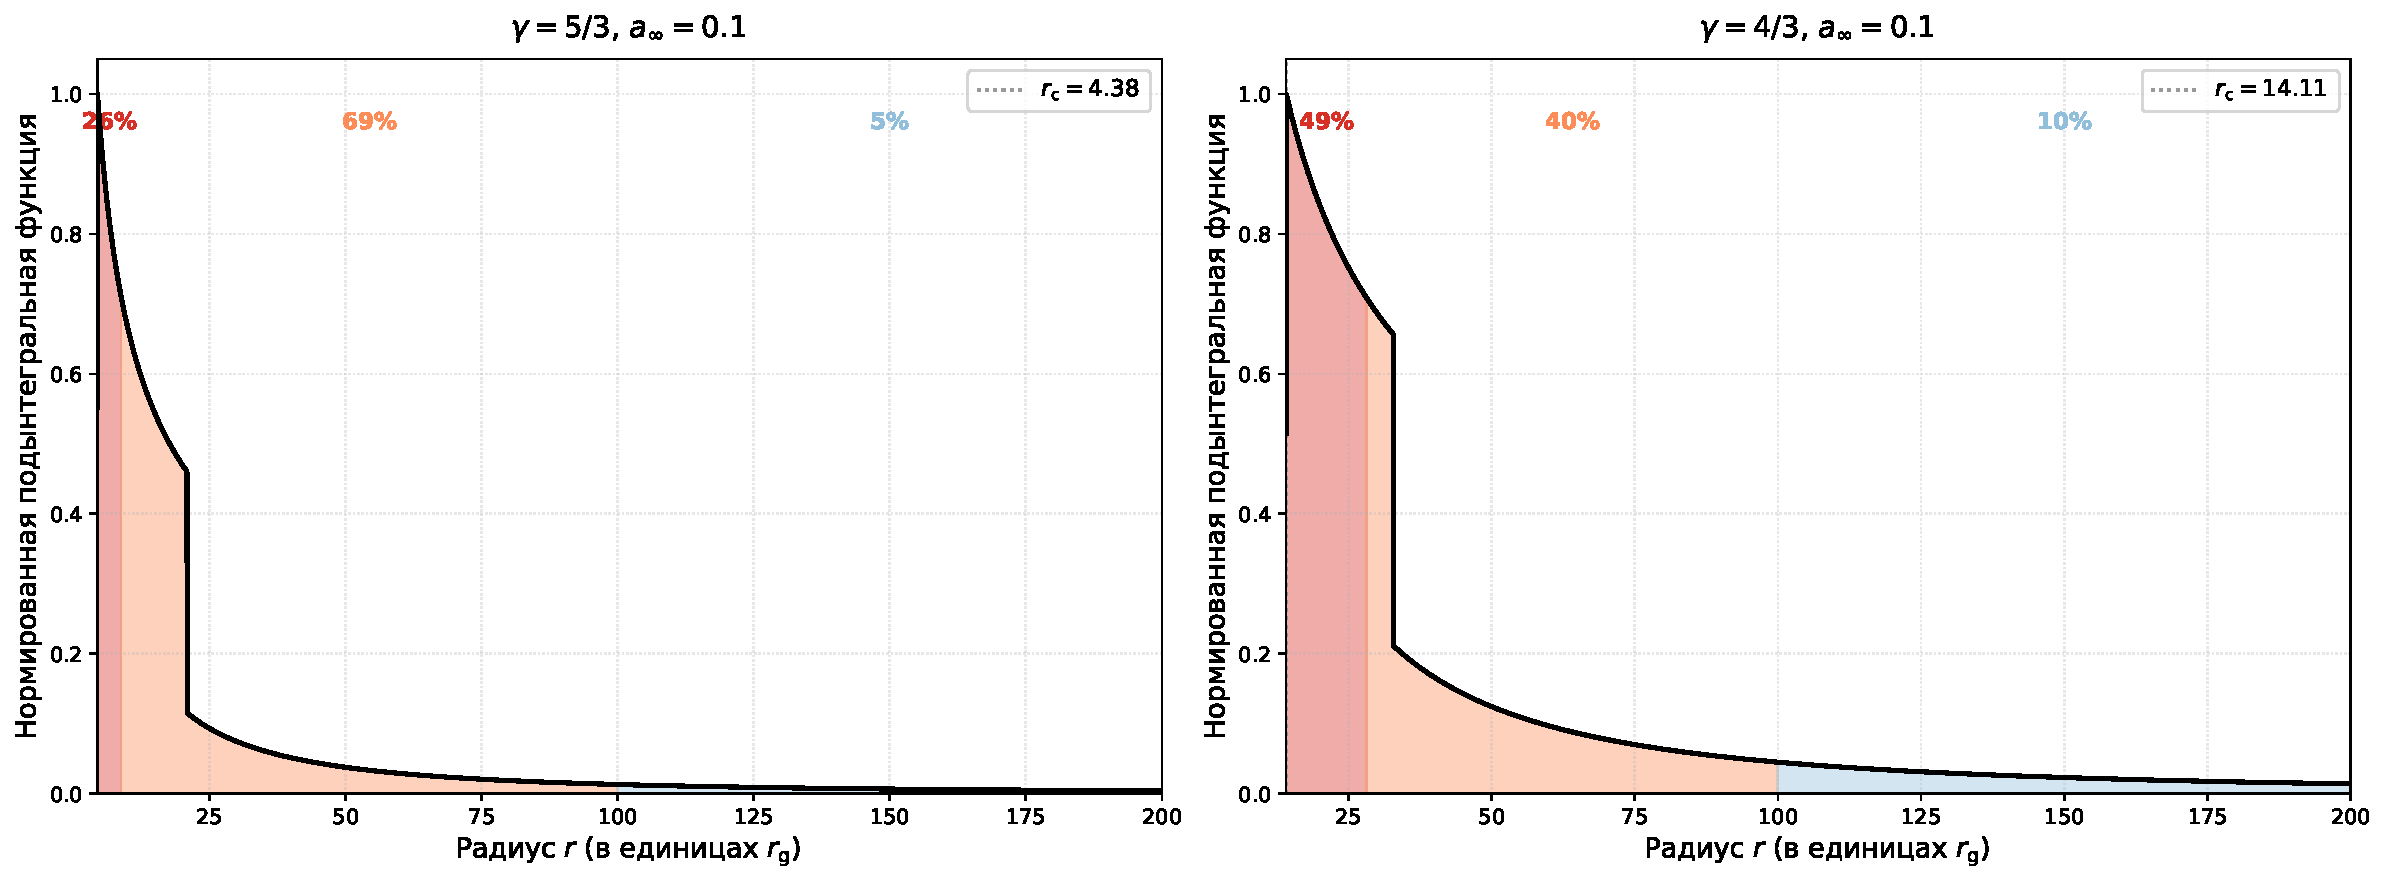
\includegraphics[width=\linewidth]{fig_inertia_localization.pdf}
                \caption{Integrand $4\pi r^{2}\rho\,\upsilon_{\mathrm{acc}}^{2}(r)$ of~\eqref{eq:effective-inertia}, normalized to its maximum value, as a function of $r$ (in units of $r_{\mathrm{g}}$) for $a_{\infty} = 0.1$. Left panel: $\gamma = 5/3$; right panel: $\gamma = 4/3$. The shaded regions highlight the contributions of three radial intervals: $[r_{\mathrm{c}}, 2r_{\mathrm{a}}]$ (acoustic-horizon region), $[2r_{\mathrm{a}}, r_{\mathrm{B}}/2]$ (intermediate zone), and $[r_{\mathrm{B}}/2, r_{\mathrm{B}}]$ (outer zone). The vertical dashed line marks $r_{\mathrm{c}}$. The numerical fractions of the contribution of each interval to the total moment of inertia $I$ are indicated in the insets.}
                \label{fig:inertia-localization}
            \end{figure}

        \subsection{Nature of the energy barrier}\label{subsec:barrier-origin}
            The effective potential $V(q)$ has a maximum at $q = 0$.
            
            Direct substitution of $\upsilon(r, q) = q \cdot \upsilon_{\mathrm{acc}}(r)$ into~\eqref{eq:energy-functional} at a \emph{fixed} profile $n(r) = n_{\mathrm{acc}}(r)$ yields a quadratic dependence $E(q) = E(0) + I q^{2}/2$, which has a minimum at $q = 0$ rather than a double well with maxima at $q = \pm 1$. To obtain a potential with two minima, one must take into account the rearrangement of the profile $n(r, q)$ as $q$ varies, which requires solving the full hydrostatic equilibrium problem with account of baryon conservation and the Bernoulli condition~\eqref{eq:michel-integrals} for each value of $q$.
            
            In the simplest symmetric phenomenological model, a double-well potential is adopted:
            \begin{equation}
                V(q) = \Delta E\,(1 - q^{2})^{2},
                \label{eq:double-well-potential}
            \end{equation}
            which provides minima at $q = \pm 1$ and a maximum $V(0) = \Delta E$ at $q = 0$ (Fig.~\ref{fig:double-well-potential}).
            
            \begin{figure}[htb]
                \centering
                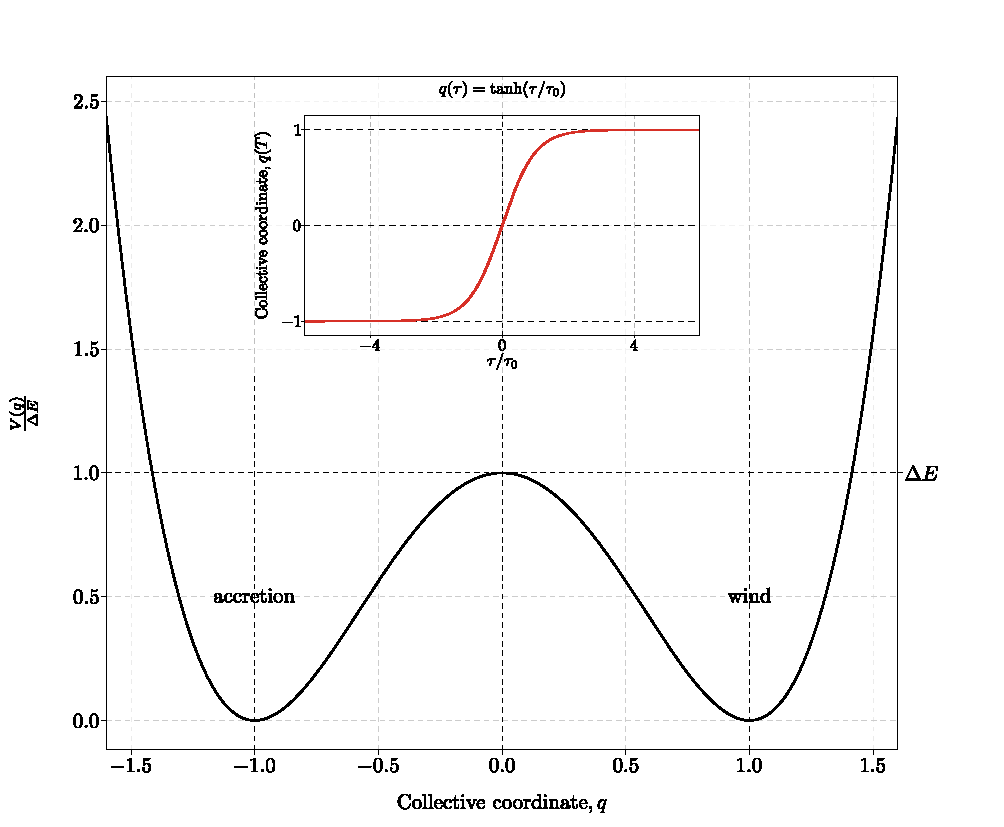
\includegraphics[width=\linewidth]{fig_double_well_potential.pdf}
                \caption{Model double-well potential $V(q) = \Delta E(1-q^{2})^{2}$ of~\eqref{eq:double-well-potential} (solid black curve); the potential $V$ is given in units of $\Delta E$, and the collective coordinate $q$ is dimensionless. The minima at $q = \pm 1$ correspond to the accretion and wind branches; the maximum $V(0) = \Delta E$ at $q = 0$ corresponds to the stopped flow. The dotted horizontal line marks the level $\Delta E$. Inset: the instanton trajectory $q(\tau) = \tanh(\tau/\tau_{0})$ as a function of the Euclidean time $\tau$ in units of $\tau_{0}$.}
                \label{fig:double-well-potential}
            \end{figure}
            
            At $q = 0$ the kinetic energy of the macroscopic flow vanishes; however, the density profile $n(r)$ and enthalpy profile $h(r)$ corresponding to the stationary flow cannot instantaneously relax to the new hydrostatic equilibrium determined by the condition $\nabla p = -(\varepsilon + p)\,\nabla\Phi_{\mathrm{eff}}$, where $\Phi_{\mathrm{eff}}$ is the effective gravitational potential (in the Newtonian limit $\Phi_{\mathrm{eff}} = -1/(2r)$). In the Schwarzschild gravitational field, the hydrostatic enthalpy profile is not homogeneous: it grows toward the center, compensating the gravitational attraction. Simultaneously, the total baryon number in the subsonic region is conserved, which imposes an integral constraint on the admissible profiles $n(r)$. It is precisely the mismatch between the inertially frozen density profile and the absence of macroscopic velocity that creates the excess energy $\Delta E$, which represents the minimal energy cost of violating the relativistic Bernoulli integral~\eqref{eq:michel-integrals} upon stopping the flow.
            
            The barrier height is estimated as the energy required to stop the flow and scales as $\Delta E \approx \alpha\, I \upsilon_{\mathrm{c}}^{2}$, where $\upsilon_{\mathrm{c}}$ is the flow velocity at the sonic point, and the dimensionless coefficient $\alpha \sim 0.3$--$0.9$ depends on the pair $(\gamma, a_{\infty})$: for $a_{\infty} = 0.1$ the coefficient is $\alpha \approx 0.31$ for $\gamma = 5/3$ and $\alpha \approx 0.52$ for $\gamma = 4/3$; for $a_{\infty} = 0.05$ the coefficient can reach $\alpha \approx 0.92$ for $\gamma = 4/3$ and decrease to $\alpha \approx 0.27$ for $\gamma = 5/3$, which reflects the enhanced dependence on the equation of state in the cold limit.

        \subsection{Instanton action}\label{subsec:instanton-action}
            The Wick rotation $\tau = it$ transforms~\eqref{eq:effective-lagrangian} into the Euclidean Lagrangian:
            \begin{equation}
                L_{\mathrm{E}} = \frac{1}{2}\,I\,\dot{q}^{\,2} + V(q).
                \label{eq:euclidean-lagrangian}
            \end{equation}
            The instanton trajectory $q(\tau)$ connects $q(-\infty) = -1$ with $q(+\infty) = +1$ and satisfies the Euclidean equation of motion:
            \begin{equation}
                I\,\ddot{q} = \frac{\mathrm{d}V}{\mathrm{d}q} = -4\Delta E\,q\,(1 - q^{2}).
                \label{eq:euclidean-eom}
            \end{equation}
            For the potential~\eqref{eq:double-well-potential}, the solution has the form:
            \begin{equation}
                q(\tau) = \tanh\left(\frac{\tau}{\tau_{0}}\right), \qquad \tau_{0} = \sqrt{\frac{I}{2\,\Delta E}}.
                \label{eq:instanton-solution}
            \end{equation}
            The instanton action is computed by integrating~\eqref{eq:euclidean-lagrangian} along~\eqref{eq:instanton-solution}:
            \begin{equation}
                \mathcal{S}_{\mathrm{inst}} = \int_{-\infty}^{+\infty} L_{\mathrm{E}}\,\mathrm{d}\tau = \int_{-1}^{+1}\sqrt{2\,I\,V(q)}\,\mathrm{d}q = \sqrt{2\,I\,\Delta E} \int_{-1}^{+1} (1 - q^{2})\,\mathrm{d}q.
                \label{eq:instanton-action-integral}
            \end{equation}
            Since elementary integration yields
            \begin{equation}
                \int_{-1}^{+1} (1 - q^{2})\,\mathrm{d}q = \left[ q - \frac{q^{3}}{3} \right]_{-1}^{+1} = \frac{4}{3},
                \label{eq:q-integral}
            \end{equation}
            the instanton action takes the finite definite form:
            \begin{equation}
                \mathcal{S}_{\mathrm{inst}} = \frac{4}{3}\sqrt{2\,I\,\Delta E}.
                \label{eq:instanton-action-final}
            \end{equation}
            This expression is finite and definite: both factors $I$ and $\Delta E$ are finite, and the action contains no divergences. Formula~\eqref{eq:instanton-action-final} is specific to the symmetric potential~\eqref{eq:double-well-potential}; for a general (not necessarily symmetric) potential $V(q)$, the instanton action is given by the integral $\mathcal{S}_{\mathrm{inst}} = \int_{-1}^{+1}\sqrt{2\,I\,V(q)}\,\mathrm{d}q$.

        \subsection{Tunneling probability and effective Planck constant}\label{subsec:tunneling-probability}
            The transition probability per unit time is given by the semiclassical formula:
            \begin{equation}
                \Gamma \sim \omega_{0}\,\exp\left(-\frac{\mathcal{S}_{\mathrm{inst}}}{\hbar_{\mathrm{eff}}}\right),
                \label{eq:tunneling-rate-final}
            \end{equation}
            where $\omega_{0} = \sqrt{V''(1)/I} = \sqrt{8\Delta E/I}$ is the frequency of small oscillations near the minimum, and $\hbar_{\mathrm{eff}}$ is the effective Planck constant of the system.

            The connection of the instanton action with the invariants of the acoustic horizon is indirect: both $\mathcal{S}_{\mathrm{inst}}$ and the formal area $\mathcal{A}_{\mathrm{a}}$ are controlled by the same macroscopic parameters $(\gamma, a_{\infty})$, as evidenced by the numerical data in Table~\ref{tab:instanton-parameters} and the values of $\kappa$ and $\mathcal{A}_{\mathrm{a}}$ tabulated in~\cite{SemyannikovAV_AcousticGeometryAndSoundRayDynamicsInRelativisticSphericalAccretion_2026}.
            
            For a classical ideal fluid, $\hbar_{\mathrm{eff}} \to 0$, and the tunneling probability is identically zero. Formula~\eqref{eq:tunneling-rate-final} acquires physical meaning only for systems with a quantum microstructure. The parameter $\hbar_{\mathrm{eff}}$ represents the ratio of a microscopic scale (e.g., the Compton wavelength of a particle $\lambda_{\mathrm{C}} = \hbar/(m c_{\mathrm{s}})$ or the coherence length in a Bose--Einstein condensate) to the macroscopic radius $r_{\mathrm{g}}$. For an astrophysical plasma ($m \sim m_{p}$, $r_{\mathrm{g}} \sim 10^{13}$ cm), the parameter $\hbar_{\mathrm{eff}} \sim 10^{-41}$, and tunneling is strictly unrealizable. For laboratory analogues (Bose--Einstein condensates, superfluid helium), $\hbar_{\mathrm{eff}}$ can reach $10^{-2}$--$10^{-4}$; however, even for $\hbar_{\mathrm{eff}} \sim 10^{-2}$ and $\mathcal{S}_{\mathrm{inst}} \sim 30$, the exponent $\exp(-\mathcal{S}_{\mathrm{inst}}/\hbar_{\mathrm{eff}}) \sim \exp(-3000)$ is vanishingly small. Tunneling of the \emph{entire} macroscopic configuration is practically unobservable under either astrophysical or laboratory conditions; the physical interest of the present result is predominantly conceptual and consists in establishing the structural analogy with vacuum black-hole--white-hole transitions~\cite{VolovikGE_PainleveGullstrandCoordinatesForSchwarzschildDeSitterSpacetime_2023}.

    \section{Discussion}\label{sec:discussion}
        \subsection{Analogy with the persistent current}\label{subsec:persistent-current}
            The structure of the problem~\eqref{eq:effective-lagrangian}--\eqref{eq:instanton-action-final} is identical to the reversal of a persistent current in a superconducting ring or a SQUID loop. The correspondence between the two systems is presented in Table~\ref{tab:analogy}.
            \begin{table}[htb]
                \centering
                \caption{Analogy between the Michel flow and a persistent current in a superconducting ring.}
                \label{tab:analogy}
                \small
                \begin{tabular}{lll}
                    \toprule
                    & Persistent current & Michel flow \\
                    \midrule
                    Degenerate states & $\pm J$ & $\upsilon < 0$ and $\upsilon > 0$ \\
                    Barrier & Inductance $LJ^{2}/2$ & Flow inertia $I$ \\
                    Collective coordinate & Phase of the order parameter $\phi$ & Degree of reversal $q$ \\
                    Instanton & Phase slip by $2\pi$ (circulation quantization) & Reversal of $\upsilon(r)$ \\
                    Suppression & $\exp(-S_{\mathrm{SQUID}}/\hbar)$ & $\exp(-\mathcal{S}_{\mathrm{inst}}/\hbar_{\mathrm{eff}})$ \\
                    Action quantum & $\hbar$ & $\hbar_{\mathrm{eff}}$ \\
                    \bottomrule
                \end{tabular}
            \end{table}
            In a superconducting ring with a Josephson junction, the Euclidean Lagrangian has the form $L_{\mathrm{E}} = \frac{1}{2}L\dot{\phi}^{2} + E_{J}(1 - \cos\phi)$, where $L$ is the inductance and $E_{J}$ is the Josephson coupling energy. For $E_{J} \ll LJ^{2}/2$, the instanton action takes the form $\mathcal{S}_{\mathrm{inst}} \approx \frac{4}{3}\sqrt{2LJ^{2}E_{J}}$, which is structurally identical to formula~\eqref{eq:instanton-action-final} under the substitution $L \to I$, $E_{J} \to \Delta E$. This correspondence shows that formula~\eqref{eq:instanton-action-final} is not an ad hoc construction but has an exact analogue in a well-studied quantum system.
            
            The key difference is that in the superconducting ring the barrier is created by the Josephson junction, whereas in the Michel flow the barrier is due to the violation of the Bernoulli integral upon stopping the flow. In both cases, the suppression is determined by the macroscopic inertia of the system.

        \subsection{Global tunneling and nucleation}\label{subsec:nucleation}
            For an infinite system, a simultaneous reversal of the entire configuration has zero probability. A physically realizable mechanism in quantum field theory is the nucleation of a bubble of the new phase~\cite{ColemanS_AspectsOfSymmetry_1985}:
            \begin{equation}
                S_{\mathrm{bubble}}(R) = 4\pi R^{2}\sigma - \frac{4\pi}{3}R^{3}\Delta\mathcal{E},
                \label{eq:coleman-action}
            \end{equation}
            where $\sigma$ is the surface tension of the wall and $\Delta\mathcal{E}$ is the difference of the energy densities of the two phases. For the Michel flow, standard nucleation is inapplicable for two reasons. First, $\Delta\mathcal{E} = 0$ (the branches are degenerate), and the extremum of~\eqref{eq:coleman-action} with respect to $R$ does not exist: the critical bubble radius $R_{\mathrm{c}} = 2\sigma/\Delta\mathcal{E}$ diverges, and the nucleation action $S_{\mathrm{bubble}} \to \infty$. Second, the wind branch is unstable: a seed of the wind configuration is immediately destroyed owing to the infinite blueshift at the white-hole horizon~\cite{SemyannikovAV_GlobalAcousticGeometryOfMichelFlowInPainleveGullstrandCoordinates_2026}.
            
            Global tunneling~\eqref{eq:tunneling-rate-final} is a correct formulation for a finite system of radius $r_{\mathrm{B}}$. The Bondi radius serves as a natural cutoff rendering the problem finite-dimensional. The probability~\eqref{eq:tunneling-rate-final} is finite but exponentially suppressed by the factor $\exp(-\mathcal{S}_{\mathrm{inst}}/\hbar_{\mathrm{eff}})$.

        \subsection{Prefactor and the negative mode}\label{subsec:prefactor}
            The prefactor $\omega_{0}$ in~\eqref{eq:tunneling-rate-final} is formally determined by the ratio of the functional determinants of fluctuations about the instanton and about the vacuum~\cite{ColemanS_AspectsOfSymmetry_1985}:
            \begin{equation}
                \omega_{0} \sim \left|\frac{\det'\bigl[-\partial_{\tau}^{2} + V''(q_{\mathrm{inst}})\bigr]}{\det\bigl[-\partial_{\tau}^{2} + V''(q_{\mathrm{vac}})\bigr]}\right|^{-1/2},
                \label{eq:prefactor-determinant}
            \end{equation}
            where the prime on $\det'$ denotes the exclusion of the zero modes and the negative mode of the instanton. The determinant receives contributions from all three families of perturbations of the Michel flow --- acoustic, vortical, and entropy modes~\cite{SemyannikovAV_PerturbationSpectrumOfMichelFlowAcousticVorticalAndEntropyModes_2026}.
            
            The physical meaning of the excluded modes is standard~\cite{ColemanS_AspectsOfSymmetry_1985}. The zero mode corresponds to the translational invariance of the instanton in time: the shift $\tau \to \tau + \tau_{0}$ does not change the action and generates a continuous family of equivalent trajectories. The negative mode (imaginary frequency) corresponds to the instability of the saddle point $q = 0$ and is responsible for the very fact of decay: the presence of exactly one negative mode is a necessary condition for the applicability of Coleman's formula for the decay rate and ensures the finiteness and positivity of the tunneling probability.

        \subsection{Connection with the surface gravity and quasinormal modes}\label{subsec:kappa-connection}
            The surface gravity $\kappa$, computed in~\cite{SemyannikovAV_AcousticGeometryAndSoundRayDynamicsInRelativisticSphericalAccretion_2026}, determines the characteristic ringdown time scale: $\tau_{\mathrm{QNM}} \sim \kappa^{-1}$. The instanton duration~\eqref{eq:instanton-solution} is $\tau_{0} = \sqrt{I/(2\Delta E)}$.
            
            From Table~\ref{tab:instanton-parameters} and the values of $\kappa$ tabulated in~\cite{SemyannikovAV_AcousticGeometryAndSoundRayDynamicsInRelativisticSphericalAccretion_2026}, it follows that $\tau_{0}^{-1} \gg \kappa$ for all parameters considered: the ratio $\tau_{0}^{-1}/\kappa$ ranges from $\sim 14$ ($\gamma = 5/3$, $a_{\infty} = 0.1$) to $\sim 200$ ($\gamma = 4/3$, $a_{\infty} = 0.05$).
            \begin{figure}[htb]
                \centering
                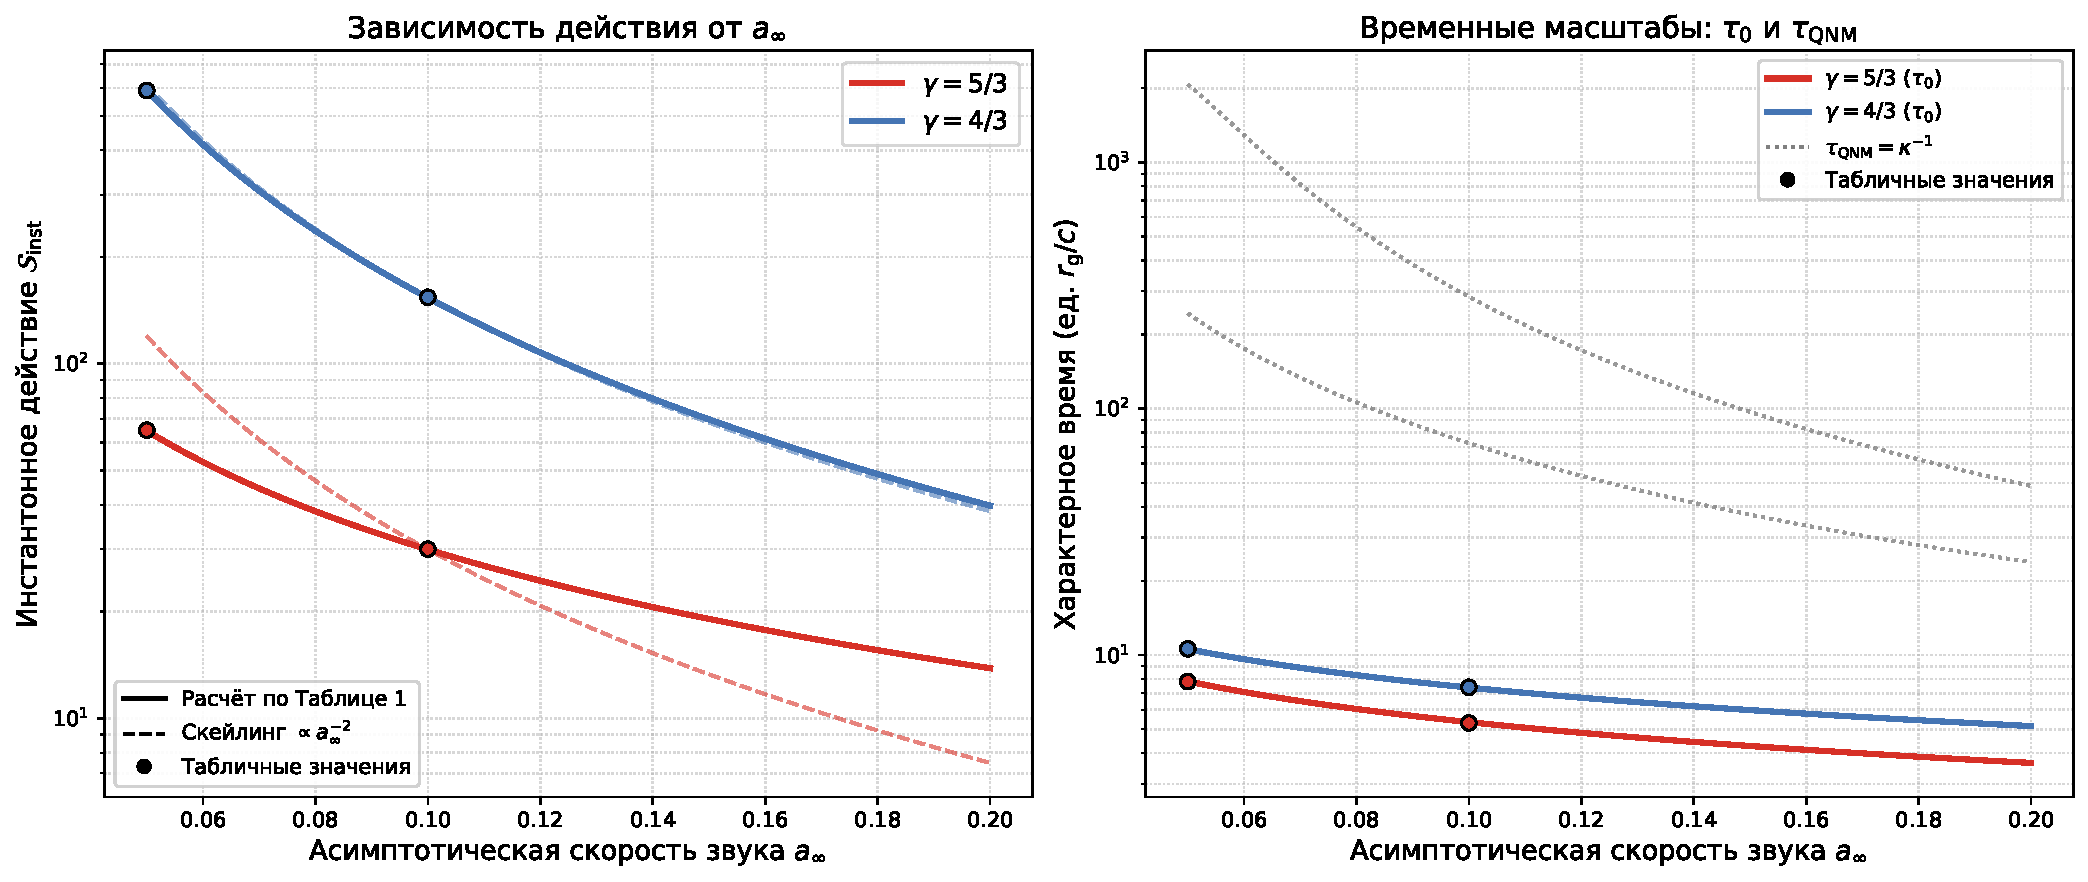
\includegraphics[width=0.88\linewidth]{fig_instanton_scaling.pdf}
                \caption{Dependence of the instanton action and the characteristic time scales on the asymptotic sound speed $a_{\infty}$. Left panel: the instanton action $\mathcal{S}_{\mathrm{inst}}$ computed from formulas~\eqref{eq:instanton-action-final} and~\eqref{eq:instanton-solution} using the values of $I$ and $\Delta E$ from Table~\ref{tab:instanton-parameters} (solid curves; markers --- tabulated values at $a_{\infty} = 0.05$ and $0.10$); dashed curves --- the approximate reference scaling $\propto a_{\infty}^{-2}$ normalized at the point $a_{\infty} = 0.1$. Right panel: the characteristic instanton time $\tau_{0} = \sqrt{I/(2\Delta E)}$ (solid curves; markers --- tabulated values) and the ringdown time $\tau_{\mathrm{QNM}} = \kappa^{-1}$, where $\kappa$ is taken from Table~2 of the companion study~\cite{SemyannikovAV_AcousticGeometryAndSoundRayDynamicsInRelativisticSphericalAccretion_2026}. Over the entire range studied, $\tau_{0} \ll \tau_{\mathrm{QNM}}$, which confirms the scale separation $\tau_{0}^{-1} \gg \kappa$.}
                \label{fig:instanton-scaling}
            \end{figure}
            This means that the instanton lasts significantly less than one period of a quasinormal mode, and the acoustic modes are \emph{frozen} on the instanton time scale (sudden approximation).
            \begin{table}[htb]
                \centering
                \caption{Numerical estimates of the instanton parameters. The values of $r_{\mathrm{c}}$ and $a_{\mathrm{c}}$ are taken from~\cite{SemyannikovAV_AcousticGeometryAndSoundRayDynamicsInRelativisticSphericalAccretion_2026}; the parameters $I$, $\Delta E$, $\mathcal{S}_{\mathrm{inst}}$, and $\tau_{0}$ are computed from formulas~\eqref{eq:effective-inertia}, \eqref{eq:double-well-potential}, \eqref{eq:instanton-action-final}, and~\eqref{eq:instanton-solution}.}
                \label{tab:instanton-parameters}
                \small
                \begin{tabular}{lcccccc}
                    \toprule
                    $\gamma$ & $a_{\infty}$ & $r_{\mathrm{c}}$ & $I$ & $\Delta E$ & $\mathcal{S}_{\mathrm{inst}}$ & $\tau_{0}$ \\
                    \midrule
                    $5/3$ & $0.05$ & $8.13$ & $3.8 \cdot 10^{2}$ & $3.1$ & $65$ & $7.8$ \\
                    $5/3$ & $0.10$ & $4.38$ & $1.2 \cdot 10^{2}$ & $2.1$ & $30$ & $5.3$ \\
                    \midrule
                    $4/3$ & $0.05$ & $51.67$ & $4.7 \cdot 10^{3}$ & $21$ & $590$ & $10.6$ \\
                    $4/3$ & $0.10$ & $14.11$ & $8.5 \cdot 10^{2}$ & $7.8$ & $154$ & $7.4$ \\
                    \bottomrule
                \end{tabular}
            \end{table}
            
            For a colder flow ($\gamma = 4/3$), the acoustic horizon is located farther out ($r_{\mathrm{c}} \approx 14.11$ versus $4.38$ at $a_{\infty} = 0.1$), which leads to a larger moment of inertia and, accordingly, to a larger instanton action. Decreasing $a_{\infty}$ from $0.1$ to $0.05$ increases $r_{\mathrm{c}}$ and, consequently, $\mathcal{S}_{\mathrm{inst}}$, which confirms the growth of the tunneling suppression in the cold limit (Fig.~\ref{fig:instanton-scaling}). This means that tunneling is more strongly suppressed for colder flows, in agreement with physical intuition: the farther the horizon, the larger the mass of fluid that must be stopped and reversed.

        \subsection{Limits of applicability}\label{subsec:limitations}
            The present analysis relies on the following limitations.
            
            First, the one-parameter reduction assumes that the transition is described by a single collective coordinate $q$. The full hydrodynamic problem contains infinitely many degrees of freedom, and the instanton trajectory in the full configuration space may differ from~\eqref{eq:instanton-solution}. Formula~\eqref{eq:instanton-action-final} provides an estimate of the action; the exact value requires solving the full Euclidean problem. The applicability criterion of the reduction demands that all other modes be heavy compared with the mode $q$, i.e., their characteristic frequencies must satisfy $\omega_{n} \gg \tau_{0}^{-1}$. For the acoustic modes this condition holds ($\tau_{0}^{-1} \gg \kappa$); however, for the advected vortical and entropy modes the scale separation becomes less pronounced: in the extended Newtonian shell outside the receding horizon their characteristic frequencies are small, and for colder flows ($a_{\infty} \lesssim 0.05$) formula~\eqref{eq:tunneling-rate-final} yields only an estimate.
            
            Second, the effective potential~\eqref{eq:double-well-potential} is model-dependent. The exact form of $V(q)$ requires a numerical solution of the hydrostatic equilibrium problem at each value of $q$, which lies beyond the scope of the present work.
            
            Third, the regularization is not uniform in the cold limit: as $a_{\infty} \to 0$ the horizon recedes to infinity ($r_{\mathrm{a}} \to \infty$), the Bondi radius diverges, and the problem loses its finite-dimensional character.
            
            Fourth, the analysis is limited to an ideal fluid without dissipation. Accounting for dissipative processes (viscosity, thermal conductivity) would lead to the appearance of a friction term of the type $-\gamma_{\mathrm{diss}}\,\dot{q}$ in the effective equation of motion (Caldeira--Leggett model), which would further suppress the tunneling probability and render the estimate~\eqref{eq:tunneling-rate-final} an upper bound.
            
            Fifth, the detailed balance between the forward and reverse transitions is broken. The wind branch is classically unstable~\cite{SemyannikovAV_GlobalAcousticGeometryOfMichelFlowInPainleveGullstrandCoordinates_2026}: ingoing perturbations experience an infinite blueshift at the horizon, which leads to an exponential growth of their energy and to the destruction of the stationary profile. The reverse process represents a fast classical decay over a time $\tau_{\mathrm{decay}} \sim \kappa^{-1}$, rather than tunneling. In a Bose--Einstein condensate, the decay of the white hole would manifest as a burst of phonon emission of duration $\sim\kappa^{-1}$ following the tunneling event.

    \section{Conclusions}\label{sec:conclusions}
        Macroscopic quantum tunneling between the acoustic black and white holes in the Michel flow has been formulated within a one-parameter model reduction. The two flow branches are degenerate stationary points of the energy functional~\eqref{eq:energy-functional}; the barrier between them is of inertial--kinematic nature and is due to the necessity of stopping and reversing the macroscopic flow. The instanton trajectory~\eqref{eq:instanton-solution} connects the two branches through the saddle point $q = 0$ in Euclidean time, and the instanton action~\eqref{eq:instanton-action-final} is expressed through the effective moment of inertia~\eqref{eq:effective-inertia} and the height of the model barrier~\eqref{eq:double-well-potential}.
        
        Numerical estimates for $a_{\infty} \in \{0.05,\, 0.1\}$ show that the instanton action is controlled by the macroscopic scales of the acoustic horizon and grows as $a_{\infty}$ decreases. The transition probability~\eqref{eq:tunneling-rate-final} is exponentially suppressed and acquires physical meaning only for systems with a quantum microstructure ($\hbar_{\mathrm{eff}} > 0$). For an astrophysical plasma, $\hbar_{\mathrm{eff}} \sim 10^{-41}$, and tunneling is strictly unrealizable; for laboratory analogues, $\hbar_{\mathrm{eff}}$ can reach $10^{-2}$--$10^{-4}$, yet tunneling of the entire macroscopic configuration remains practically unobservable. The detailed balance between the forward and reverse transitions is broken: the wind branch is classically unstable, and the reverse process represents a fast decay over a time $\tau_{\mathrm{decay}} \sim \kappa^{-1}$, rather than tunneling. Coleman nucleation is inapplicable owing to the degeneracy of the branches ($\Delta\mathcal{E} = 0$) and the instability of the seed.
        
        Natural extensions of the work include the following directions. First, a numerical computation of the exact form of $V(q)$ by solving the hydrostatic equilibrium problem at each value of $q$ would yield exact values of $\Delta E$ and $\mathcal{S}_{\mathrm{inst}}$. Second, a 3+1 decomposition of the acoustic core in the ADM form would allow the analog Hawking temperature and its redshift to be derived, providing a direct connection between the macroscopic tunneling and the kinematic Hawking radiation~\cite{VolovikGE_PainleveGullstrandCoordinatesForSchwarzschildDeSitterSpacetime_2023}. Third, the inclusion of non-adiabatic flow, rotation, and backreaction of perturbations on the background would extend the analysis to more realistic astrophysical settings. Fourth, reversing the sign of the flow velocity to realize an acoustic white hole~\cite{SemyannikovAV_GlobalAcousticGeometryOfMichelFlowInPainleveGullstrandCoordinates_2026} would allow the time-reversed tunneling process to be investigated. Fifth, since the instanton describes a global reversal of the configuration whereas Hawking radiation is a local process at the horizon, it is of interest whether the vacuum Hawking fluctuations can serve as a seed for initiating the white-hole instability immediately after tunneling.

    \section*{Acknowledgments}
        The work was performed by an independent researcher without institutional funding. The NASA Astrophysics Data System database was used in the preparation.

    \bibliographystyle{elsarticle-num}
    \bibliography{article}
\end{document}